%# -*- coding: utf-8-unix -*-
%%==================================================
%% chapter01.tex for SJTU Master Thesis
%%==================================================

%\bibliographystyle{sjtu2}%[此处用于每章都生产参考文献]
\chapter{一种基于自适应滑模方法的抗参数扰动的容错控制策略}
\label{chap:asmcsat}
\section{引言}
作为一种轻于空气的飞行器,浮空器在平流层的稳定能力是评价其性能的重要标准。然而,如第\newref{chap:preliminary}章所介绍,浮空器特有的高附加质量和气动参数不准确问题,给它的稳定控制增加了很大的困难。在近期的研究中,曾经有针对航空器采用自适应控制的策略应对质量矩阵不确定性的研究,如\cite{7061535}。文献\cite{7978124}针对浮空器不停变化的气动力设计了一个非线性扰动观测器,以此来抵消气动系数不确定的影响。但是目前在浮空器上同时考虑质量矩阵不确定和气动系数的研究仍然缺乏。本章结合了自适应控制与滑模控制各自的优点,提出了一种新的自适应率,并设计了一种新的容错控制器,能够使得浮空器在质量矩阵扰动和气动系数扰动都未知的情况下仍然保持姿态和位置稳定。同时,考虑到实际情况,还引入了一种执行机构抗饱和策略。

\section{问题表述}
式\neweqref{eq:model1}所示的浮空器模型如下
\begin{equation*}
    \begin{cases}
    \dot{\mathbf{x}}_1 &= \mathbf{J}\mathbf{x}_2 \\
    \mathbf{M}\dot{\mathbf{x}}_2 &= \mathbf{F_{gb}} + \mathbf{F_a} + \mathbf{F_i} + \mathbf{F_t}
    \end{cases}
\end{equation*}

为了书写方便,这里将气动力矩阵$\mathbf{F_a}$写成参数分离的形式,即
\begin{equation}\label{eq:Fa-para}
    \mathbf{F_a} = \mathbf{S}(\mathbf{x}_2)\mathbf{c}
\end{equation}
其中
\begin{equation}\label{eq:Sx2}
\mathbf{S(x_2)}=\left[
\begin{matrix}
q_\infty\cdot S_{ref}\cdot\cos\Omega&0&0 \\
q_\infty\cdot S_{ref}\cdot\sin\Omega&0&0  \\
0&q_\infty\cdot S_{ref}&0  \\
0&0&-q_\infty\cdot S_{ref}\cdot L_{ref}\cdot \cos\Omega  \\
0&0&-q_\infty\cdot S_{ref}\cdot L_{ref}\cdot \sin\Omega  \\
0&0&0  \\
\end{matrix}
\right]
\end{equation}

\begin{equation}\label{eq:cvector}
    \mathbf{c} = \left[\begin{matrix}
    C_x&C_z&C_{my}
    \end{matrix}\right]^T
\end{equation}

质量矩阵和气动系数都不缺定的情况,表现在模型中,可以假设为
\begin{eqnarray}
    \mathbf{M}&=&\mathbf{M}+\mathbf{M}_{\Delta} \label{eq:Muncertainty} \\
    \mathbf{c}&=&\mathbf{c}+\mathbf{c}_{\Delta} \label{eq:cuncertainty}
\end{eqnarray}

其中$\mathbf{M}_{\Delta}$和$\mathbf{c}_{\Delta}$都是未知扰动。

新的浮空器模型变为
\begin{equation}\label{eq:modelwc}
    \begin{cases}
    \hspace{4.5em}\dot{\mathbf{x}}_1 &= \mathbf{J}\mathbf{x}_2\\
    (\mathbf{M}+\mathbf{M}_{\Delta})\dot{\mathbf{x}}_2&=\mathbf{F_{gb}+F_{i}(x_2)}+\mathbf{S(x_2)} (\mathbf{c}+\mathbf{c}_{\Delta})+\mathbf{F_t}
    \end{cases}
\end{equation}

本章任务是针对浮空器模型\neweqref{eq:modelwc}提出一种控制策略使其保持姿态和位置。

\section{算法详述与稳定性证明}\label{sec:3algo}
为了表述方便,下文用函数$\mathbf{F}(\mathbf{x}_1,\mathbf{x}_2)$指代$\mathbf{F_{gb}+F_{i}(x_2)}+\mathbf{S(x_2)} (\mathbf{c}+\mathbf{c}_{\Delta})$。飞艇的动力学方程变为
\begin{equation}\label{eq:dynamicwc}
    (\mathbf{M}+\mathbf{M}_{\Delta})\dot{\mathbf{x}}_2=\mathbf{F(x_1,x_2)+u}
\end{equation}

选择滑模面
\begin{equation}
    \mathbf{s}(t)=\mathbf{x_2+Cx_1}=0
\end{equation}

这里$\mathbf{C}\in\mathbb{R}^{6\times 6}>0$是收敛参数。在给出控制率之前,我们需要做如下几个假设

\begin{ass}\label{3ass:M}
添加了扰动后的质量矩阵是正定的,并且有一个未知的上限$M_{max}$,不会趋近于无穷大。即
\begin{equation}\label{eq:3assM}
    \lVert\mathbf{M}+\mathbf{M}_{\Delta}\rVert\leqslant M_{max}
\end{equation}
\end{ass}
\begin{ass}\label{3ass:F}
浮空器的重浮力、科氏力和气动力的合力满足
\begin{equation}\label{eq:3assF}
    \bnorm{F(x_1,x_2)}\leqslant k_0+k_1\bnorm{x_1}+k\bnorm{x_2}
\end{equation}
其中$k_0$, $k_1$, $k$为正实数。
\end{ass}
根据假设\newref{3ass:M},可以再做出一个合理假设
\begin{ass}\label{3ass:MCJ}
惯性矩阵$\mathbf{M}$, 惯性矩阵的扰动$\mathbf{M}_{\Delta}$, 滑模面参数矩阵$\mathbf{C}$, 坐标转换矩阵$\mathbf{J}$满足:
\begin{equation}
    \lVert(\mathbf{M}+\mathbf{M}_{\Delta})\mathbf{CJ}\rVert\bnorm{x_2}\leqslant (k_2-k)\bnorm{x_2}
\end{equation}
其中$k_2>k$为正实数。
\end{ass}

\begin{rem}
上述假设\newref{3ass:M}-\newref{3ass:MCJ}都是合理的。对于假设\newref{3ass:M},由于浮空器的惯性矩阵$\mathbf{M}$本身在无附加质量的情况下是正定的,只要附加质量不超过浮空器质量本身,假设\newref{3ass:M}都是能够成立的。而附加质量如果超过质量本身的情况,需要更加复杂的分析,本章不做讨论;假设\newref{3ass:F}和假设\newref{3ass:MCJ}给出的条件都是给不确定性设置了一个上界,不同于传统方法设置常值上界,这里采用浮空器自身的状态变量来设置这个上界,浮空器状态变量的值越大,那么浮空器受到的不确定性也越大,符合实际条件。假设\newref{3ass:F}和\newref{3ass:MCJ}中,假定不确定性的增长不快于浮空器状态变量的线性增长,是为了方便后文的推导。如果选择一些多项式函数或者非线性函数,也可以通过重新选取滑模面或自适应率达到同样的效果。
\end{rem}

基于假设\newref{3ass:M}-\newref{3ass:MCJ},定义控制输入$\mathbf{u}$为
\begin{equation}\label{eq:3input}
\mathbf{u} = -\tau\mathbf{s}(t)-\sigma \mathrm{sign}\,(\mathbf{s}(t)) - \mathbf{u_p}
\end{equation}

其中
\begin{eqnarray}
    \tau &=& \left[\begin{matrix}
         \tau_1&&  \\
         &\ddots& \\
         &&\tau_6
    \end{matrix}\right] \\
    \sigma &=& \left[\begin{matrix}
         \sigma&&  \\
         &\ddots& \\
         &&\sigma
    \end{matrix}\right] \\
    \hat{\rho}&=&\hat{k_0}+\hat{k_1}\bnorm{x_1}+\hat{k_2}\bnorm{x_2} \label{eq:inputrho} \\
    \dot{\hat{k_0}}&=&p_0\bnorm{s} \label{eq:adlaw1} \\
    \dot{\hat{k_1}}&=&p_1\bnorm{s}\bnorm{x_1} \label{eq:adlaw2} \\
    \dot{\hat{k_2}}&=&p_2\bnorm{s}\bnorm{x_2} \label{eq:adlaw3}
\end{eqnarray}

\begin{rem}
控制器\neweqref{eq:3input}由三个部分组成。$\mathbf{u_p}$是用于补偿不确定性的自适应率。$-\tau\mathbf{s}(t)-\sigma \mathrm{sgn}(\mathbf{s}(t))$ 这两项能够保证系统到达滑模面并且持续留在滑模面上。$\tau$和$\sigma$是设计参数,用于控制系统到达滑模面的时间。理论上不论是$-\tau\mathbf{s}(t)$还是$-\sigma \mathrm{sgn}(\mathbf{s}(t))$都足够保证系统的收敛,本文设计控制器的时候流出了一部分冗余参数以适应一些未知情况,也能保证让系统状态更快地收敛到滑模面上。
\end{rem}

下面将证明控制器\neweqref{eq:3input}能够在基于假设\newref{3ass:M}-\newref{3ass:MCJ}的条件下,使得浮空器系统\neweqref{eq:modelwc}稳定。

选取李雅普诺夫函数
\begin{equation}\label{eq:3lyapnov}
    V=\frac{1}{2}\left[\mathbf{s}^T(\mathbf{M}+\mathbf{M}_{\Delta})\mathbf{s}+\frac{1}{p_0}(k_0-\hat{k_0})^2+\frac{1}{p_1}(k_1-\hat{k_1})^2+\frac{1}{p_2}(k_2-\hat{k_2})^2\right]
\end{equation}

对$V$求导,得到
\begin{align}\label{eq:Vdot}
    \dot{V}&=\mathbf{s}^T(\mathbf{M}+\mathbf{M}_{\Delta})\mathbf{s}-\frac{1}{p_0}(k_0-\hat{k_0})\dot{\hat{k_0}}-\frac{1}{p_1}(k_1-\hat{k_1})\dot{\hat{k_1}}-\frac{1}{p_2}(k_2-\hat{k_2})\dot{\hat{k_2}} \nonumber
\\&=\mathbf{s}^T(\mathbf{M}+\mathbf{M}_{\Delta})\mathbf{(C\dot{x}_1+\dot{x}_2)} - \Delta \nonumber
\\&=\mathbf{s}^T(\mathbf{M}+\mathbf{M}_{\Delta})\mathbf{Cx_2}+\mathbf{{s^{T}[F(x_1,x_2)+u]}}-\Delta \nonumber
\\& \leqslant \mathbf{\norm{s}\norm{(M+M_{\Delta})C}\norm{x_2}+\norm{s}\norm{F(x_1,x_2)}}+\mathbf{s^{T}u}-\Delta \nonumber
\\& \leqslant \bnorm{s}[(k_2-k)\norm{\mathbf{x_2}}+(k_0+k_1\norm{\mathbf{x_1}}+k\norm{\mathbf{x_2}})]+\mathbf{s^{T}u}-\Delta \nonumber
\\&=\norm{\mathbf{s}}(k_0+k_1\norm{\mathbf{x_1}}+k_2\norm{\mathbf{x_2}})+\mathbf{s^{T}u}-\Delta 
\end{align}

为书写方便,式\neweqref{eq:Vdot}中
\begin{equation}\label{eq:Delta}
    \Delta = -\frac{1}{p_0}(k_0-\hat{k_0})\dot{\hat{k_0}}-\frac{1}{p_1}(k_1-\hat{k_1})\dot{\hat{k_1}}-\frac{1}{p_2}(k_2-\hat{k_2})\dot{\hat{k_2}}
\end{equation}

注意到
\begin{align}\label{eq:process1}
&\mathbf{s}^T\mathbf{u}-\Delta \nonumber
\\&= \mathbf{s}^T\Big[-\tau\mathbf{s}-\sigma\mathrm{sign}\,(\mathbf{s})-\frac{\mathbf{s}}{\bnorm{s}}(\hat{k_0}+\hat{k_1}\bnorm{x_1}+\hat{k}\bnorm{x_2})\Big]-\Delta \nonumber
\\&=\mathbf{s}^T[-\tau \mathbf{s}-\sigma\mathrm{sgn}(\mathbf{s})]-\bnorm{s}(\hat{k_0}+\hat{k_1}\bnorm{x_1}+\hat{k_2}\bnorm{x_2})-\Delta
\end{align}

设$s_i$为滑模面向量$\mathbf{s}$的各个分量,把\neweqref{eq:Delta}、\neweqref{eq:process1}代入\neweqref{eq:Vdot},可以得到
\begin{align}\label{eq:V<03-1}
    \dot{V}&=\mathbf{s^{T}[-\tau s-\sigma \mathrm{sgn}(s)]} \nonumber\\
    &=\sum_{i=1}^{6}-\tau_is_i^{2}-\sigma_i\abs{s_i}\leqslant0
\end{align}

证毕。
\vspace{1em}

通过\neweqref{eq:V<03-1}式,结合Barbashin-Krasovskii定理\footnote{《非线性系统》\cite{Khalilnonlinearbookchinese},Hassan K. Khalil著,电子工业出版社,2012年版,第124页}可知控制器\neweqref{eq:3input}能够在基于假设\newref{3ass:M}-\newref{3ass:MCJ}的条件下,使得浮空器系统\neweqref{eq:modelwc}稳定。以下推导中$\mathbf{u}$即表示所需控制输入量$\mathbf{F_t}$。

\section{抗饱和策略的引入}\label{sec:3sat}
浮空器在运行时不可避免地会遇到执行机构饱和问题,本节在\newref{sec:3sat}的基础上,对上述控制器\neweqref{eq:3input}进行一些修改,使其能够处理执行机构饱和的问题。

首先需要对执行机构饱和进行数学建模。我们用$\mathbf{u}_{sat}$来代替实际系统考虑饱和后的输入。

此时浮空器系统变为:
\begin{equation}\label{eq:modelwcsat}
    \begin{cases}
    \hspace{4.5em}\dot{\mathbf{x}}_1 &= \mathbf{J}\mathbf{x}_2\\
    (\mathbf{M}+\mathbf{M}_{\Delta})\dot{\mathbf{x}}_2&=\mathbf{F_{gb}+F_{i}(x_2)}+\mathbf{S(x_2)} (\mathbf{c}+\mathbf{c}_{\Delta})+\mathbf{u}_{sat}
    \end{cases}
\end{equation}

而$\mathbf{u}_{sat}$的表达式为

\begin{equation}\label{eq:satu}
    \mathbf{u}_{sat} = \mathbf{E}\mathbf{u}
\end{equation}

这里$\mathbf{u}=[u_1,u_2,\cdots,u_6]^T$是期望输入,$\mathbf{E}$是如下对角矩阵:
\begin{equation*}
    \mathbf{E} = \left[\begin{matrix}
         \varepsilon_1&&  \\
         &\ddots& \\
         &&\varepsilon_6
    \end{matrix}\right] 
\end{equation*}
并满足
\begin{equation*}
    \varepsilon_i = \begin{cases}
    \frac{|u_{mi}|}{|u_i|} & \text{if } u_i>u_{mi}\\
    1 & \text{if } u_i \leqslant u_{mi}
    \end{cases}
\end{equation*}
$u_{mi}$是第$i$个分量的最大输入,$0<\varepsilon_i<1$。

此外,\newref{sec:3algo}节中的假设条件需要变动为如下两个假设条件:

\begin{ass}\label{3ass:sat1}
浮空器的重浮力、科氏力和气动力的合力满足
\begin{equation}\label{eq:3asssat1}
    \bnorm{F(x_1,x_2)}\leqslant m_0\bnorm{x_2}
\end{equation}
其中$m_0$为正实数。
\end{ass}

\begin{ass}\label{3ass:sat2}
惯性矩阵$\mathbf{M}$, 惯性矩阵的扰动$\mathbf{M}_{\Delta}$, 滑模面参数矩阵$\mathbf{C}$, 坐标转换矩阵$\mathbf{J}$满足:
\begin{equation}\label{eq:3asssat2}
    \lVert(\mathbf{M}+\mathbf{M}_{\Delta})\mathbf{CJ}\rVert\bnorm{x_2}\leqslant (m-m_0)\bnorm{x_2}
\end{equation}
其中$m$为正实数,并满足$m>m_0$。
\end{ass}

为证明方便,先引入如下引理
\begin{lem}\label{lm:chap3}
    若$\mathbf{x}=\left[\begin{matrix}x_1&x_2&\cdots&x_n\end{matrix}\right]^T$是一个$n\times 1$的向量,$A$是一个$n\times n$的对角矩阵且满足$A=diag(a_1,a_2,\cdots,a_n)\text{,}(0<a_i<1)$。$k$是一个正实数标量,$a_{low}$是$a_1,\cdots,a_n$中最小的元素,那么有如下结论:
    \begin{equation}
        \mathbf{x}^TAk\mathbf{x}\geqslant ka_{low}\bnorm{\mathbf{x}}^2
    \end{equation}
\end{lem}

\begin{proof}
    \begin{align}
    \mathbf{x}^TAk\mathbf{x} &= \sum_{i=1}^n ka_ix_i^2 \nonumber\\
    &\geqslant \sum_{i=1}^n ka_{low}x_i^2 \nonumber\\
    &= ka_{low}\sum_{i=1}^n x_i^2 \nonumber\\
    &= ka_{low}\bnorm{\mathbf{x}}^2  
    \end{align}
    证毕。
\end{proof}

根据假设\newref{3ass:sat1}和\newref{3ass:sat2},定义控制率

\begin{equation}\label{eq:inputsat}
\mathbf{u}_{sat} = -\tau\mathbf{s}(t)-\sigma \mathrm{sign}\,(\mathbf{s}(t)) - \mathbf{u_s}
\end{equation}

其中
\begin{eqnarray}
        \tau &=& \left[\begin{matrix}
         \tau_1&&  \\
         &\ddots& \\
         &&\tau_6
    \end{matrix}\right] \nonumber\\
    \sigma &=& \left[\begin{matrix}
         \sigma&&  \\
         &\ddots& \\
         &&\sigma
    \end{matrix}\right] \nonumber\\
    \mathbf{u_s}&=&\frac{\hat{\beta}\hat{m}\bnorm{x_2}\mathbf{s}}{\bnorm{s}} \\
    \dot{\hat{m}} &=& p_3\bnorm{s}\bnorm{x_2} \label{eq:updatead1} \\
    \dot{\hat{\beta}} &=& \hat{\beta}^3\hat{m}\bnorm{s}\bnorm{x_2} \label{eq:updatead2}
\end{eqnarray}

下面证明,控制率\neweqref{eq:inputsat}在假设\newref{3ass:sat1}和\newref{3ass:sat2}的条件下,能够使得浮空器饱和输入模型\neweqref{eq:modelwcsat}保持稳定。

首先,选取一个标量$\xi$满足
\begin{equation}\label{eq:choosexi}
    0<\xi<\mbox{min}\{\varepsilon_1,\varepsilon_2,\cdots,\varepsilon_6\}<1
\end{equation}

定义李雅普诺夫函数
\begin{equation}\label{eq:lyapads}
    V_s=\frac{1}{2}\left[\mathbf{s^T(M+M_{\Delta})s}+\frac{1}{p_3}\tilde{m}^2+\frac{1}{p_4}\tilde{\beta}^2\right]
\end{equation}
其中$\tilde{m}=m-\hat{m}$,$\tilde{\beta}=\xi-\frac{1}{\hat{\beta}}$。

显然可得$\dot{\tilde{m}}=-\dot{\hat{m}}$ 和 $\dot{\tilde{\beta}}=\frac{\dot{\hat{\beta}}}{\hat{\beta}^2}$

对$V_s$求导,得到
\begin{align}
    \dot{V}_s &= \mathbf{s}^T(\mathbf{M}+\mathbf{M}_{\Delta})\mathbf{s} + \frac{1}{p_3}\tilde{m}\dot{\tilde{m}}+\frac{1}{p_4}\tilde{\beta}\hat{\tilde{\beta}} \nonumber\\
&=\mathbf{s}^T(\mathbf{M}+\mathbf{M}_{\Delta})\mathbf{(\dot{x}_2+Cx_2)}-\frac{\tilde{m}\dot{\hat{m}}}{p_3}+\frac{\tilde{\beta}\dot{\hat{\beta}}}{p_4\hat{\beta}^2} \nonumber\\
&= \mathbf{s}^T(\mathbf{M}+\mathbf{M}_{\Delta})\mathbf{Cx_2}+\mathbf{s^T}(\mathbf{F}+\mathbf{u}_{sat})-\tilde{m}\bnorm{s}\bnorm{x_2}+\tilde{\beta}\hat{\beta}\hat{m}\bnorm{s}\bnorm{x_2} \nonumber\\
&\leqslant \bnorm{s}(m-m_0)\bnorm{x_2}+m_0\bnorm{s}\bnorm{x_2}+\mathbf{s^TEu}-\tilde{m}\bnorm{s}\bnorm{x_2}+\tilde{\beta}\hat{\beta}\hat{m}\bnorm{s}\bnorm{x_2} \nonumber\\
&=\mathbf{s^TE}(-\tau\mathbf{s}(t)-\sigma \mathrm{sign}\,(\mathbf{s}(t)) - \mathbf{u_s})+\hat{m}\bnorm{s}\bnorm{x_2}+\tilde{\beta}\hat{\beta}\hat{m}\bnorm{s}\bnorm{x_2} \nonumber\\
&= \mathbf{s^TE}(-\tau\mathbf{s}(t)-\sigma \mathrm{sgn}(\mathbf{s}(t)))-\mathbf{s^TEu_s}+\hat{m}\bnorm{s}\bnorm{x_2}+(\xi-\frac{1}{\hat{\beta}})\hat{\beta}\hat{m}\bnorm{s}\bnorm{x_2} \nonumber\\
&=-\sum_{i=1}^6(\varepsilon_i\tau_is_i^2-\varepsilon_i\sigma_i|s_i|)-\mathbf{s^TE}\frac{\hat{\beta}\hat{m}\bnorm{x_2}\mathbf{s}}{\bnorm{s}}+\xi\hat{\beta}\hat{m}\bnorm{s}\bnorm{x_2} \label{eq:lypaad1}
\end{align}

由引理\newref{lm:chap3},可得
\begin{align}
    \mathbf{s^TE}\frac{\hat{\beta}\hat{m}\bnorm{x_2}}{\bnorm{s}}\mathbf{s} &\geqslant \frac{\hat{\beta}\hat{m}\bnorm{x_2}}{\bnorm{s}}\varepsilon_{low}\bnorm{s}^2> \xi\hat{\beta}\hat{m}\bnorm{s}\bnorm{x_2}
\end{align}

继续由\neweqref{eq:lypaad1}得
\begin{equation}
    \dot{V}_s<-\sum_{i=1}^6(\varepsilon_i\tau_is_i^2+\varepsilon_i\sigma_i|s_i|)
\end{equation}

因为$\varepsilon_i, \sigma_i, \tau_i\text{  (i$\in$\{1,2,$\cdots$,6\})}$都是正实数,因此可得$\dot{V}_s<0$,证毕。
\vspace{1em}

因此,控制率\neweqref{eq:inputsat}在假设\newref{3ass:sat1}和\newref{3ass:sat2}的条件下,能够使得浮空器饱和输入模型\neweqref{eq:modelwcsat}保持稳定。

\section{数值仿真与对比}
在本节中,我对\newref{sec:3algo}和\newref{sec:3sat}提到的算法进行了仿真。在给出仿真结果前,表\newref{tab:para}中给出了一些必要的浮空器参数。

\begin{table}[!htp]
  \centering
  \bicaption[tab:para]{浮空器模型参数}{浮空器模型参数}{Table}{Airship model parameters}
  \vspace{0.5em}
  \begin{tabular}{cl}
    \toprule
    参数&值\\
    \midrule
    $m(kg)$&72\\
    $m_{11}(kg)$&10.8147\\
    $m_{22}(kg)$&10.8147\\
    $m_{33}(kg)$&38.9521\\
    $m_{44}(kg)$&19.3024\\
    $m_{55}(kg)$&19.3024\\
    $m_{66}(kg)$&0\\
    $I_x(kg\cdot m^2)$&409.4260\\
    $I_y(kg\cdot m^2)$&409.4260\\
    $I_z(kg\cdot m^2)$&34.5941\\
    $R_p(m)$&2.81\\
    $(x_G,y_G,z_G)(m)$&(0,0,2)\\
    \bottomrule
  \end{tabular}
\end{table}

为了更直观地说明算法的效果,本文同时也给出了D. Han论文中针对浮空器设计的自适应反演(Adaptive Backsteppting, ABS)算法\cite{han2015adaptive}和Y. Yang论文中\cite{Yang2016Positioning}针对浮空器设计的反演滑模(Backstepping Sliding Mode Control, BSMC)位置控制算法的结果进行对比。需要注意的是,Y. Yang论文中的算法是针对一个三自由度模型设计的,我们仿真的时候用它来对六自由度模型进行控制,其结果是不可预测的。

对于仿真中用到的参数说明如下:滑模参数选取为$\tau=2\mathbf{I_6}$, $\sigma=0.001\mathbf{I_6}$ 和 $\mathbf{C}=0.3\mathbf{I_6}$,其中$\mathbf{I}_6$是$6\times 6$的单位矩阵。自适应率中的参数$p_0=p_1=p_2=p_3=p_4=1$。各个自适应变量的初值为$\hat{k}_0(0)=\hat{k}_1(0)=\hat{k}_2(0)=\hat{m}(0)=\hat{\beta}(0)=0.001$。每个螺旋桨的最大推力设置为110N。本节仿真主要分为如下几个部分:
\begin{description}
    \item[仿真1:两组无参数扰动情况] 对照组,选取$\mathbf{M}_{\Delta}=\mathbf{c}_{\Delta}=0$,使用\newref{sec:3algo}节的算法、D. Han的算法以及Y. Yang的算法对两组初值进行仿真对比,仿真时长40秒。
    \item[仿真2:\newref{sec:3algo}节算法有扰动] 对于\newref{sec:3algo}节的算法,在有扰动情况下与Y. Yang和D. Han的算法进行了对比,仿真时长40秒。
    \item[仿真3:\newref{sec:3sat}节算法有扰动] 对于\newref{sec:3sat}节的算法,在有扰动情况下与Y. Yang和D. Han的算法进行了对比,仿真时长40秒。
    \item[仿真4:\newref{sec:3algo}节算法大偏移] 在仿真1-仿真3中都使用的是较小初始状态偏移量,由于自适应参数会随着仿真时长不断增大,影响到算法对于大偏移量的表现,因此在仿真4中尝试较大初始偏移,采用\newref{sec:3sat}节的算法,仿真时长200秒。
\end{description}

\subsection{仿真1:无扰动情况}\label{sec:sim3-1}
无扰动情况下,两种初始状态在表\newref{tab:initstate0s}和\newref{tab:initstate0}中给出。
\begin{table}[htp]
    \centering
    \bicaption[tab:initstate0s]{无扰动初始状态1}{无扰动初始状态1}{Table}{The initial state of the airship at $t=0$ with no disturbance: Case 1}
    \vspace{0.5em}
    \begin{tabular}{cl}
        \toprule
        状态变量&值  \\
        \midrule
        $\mathbf{P}(m)$&$[1,-2,1]^T$  \\
        $\mathbf{\Omega}$(rad)&$[\pi/6,-\pi/12,\pi/6]^T$  \\
        $\mathbf{v}$(m/s)&$[1,-1,0]^T$  \\
        $\mathbf{w}$(rad/s)&$[0.1,-0.1,0.1]^T$\\
        \bottomrule
    \end{tabular}    
\end{table}
\begin{table}[htp]
    \centering
    \bicaption[tab:initstate0]{无扰动初始状态2}{无扰动初始状态2}{Table}{The initial state of the airship at $t=0$ with no disturbance: Case 2}
    \vspace{0.5em}
    \begin{tabular}{cl}
        \toprule
        状态变量&值  \\
        \midrule
        $\mathbf{P}(m)$&$[8.5,-7,4]^T$  \\
        $\mathbf{\Omega}$(rad)&$[\pi/6,-\pi/12,\pi/3]^T$  \\
        $\mathbf{v}$(m/s)&$[1,-1.5,-1]^T$  \\
        $\mathbf{w}$(rad/s)&$[0.1,-0.2,0.1]^T$\\
        \bottomrule
    \end{tabular}    
\end{table}

\begin{figure}[!h]
    \centering
    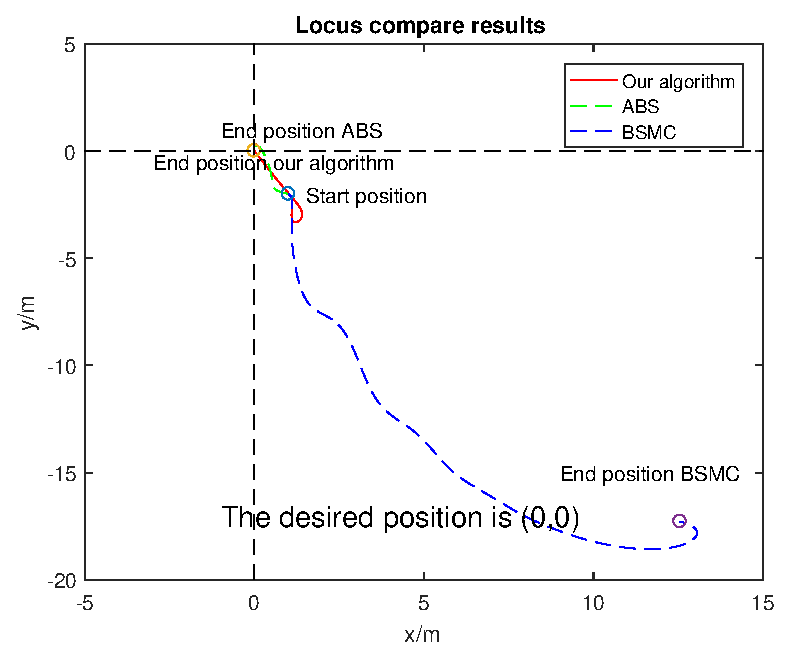
\includegraphics[width=0.45\textwidth]{figure/chap03/case0s-locus.eps}
    \hspace{1em}
    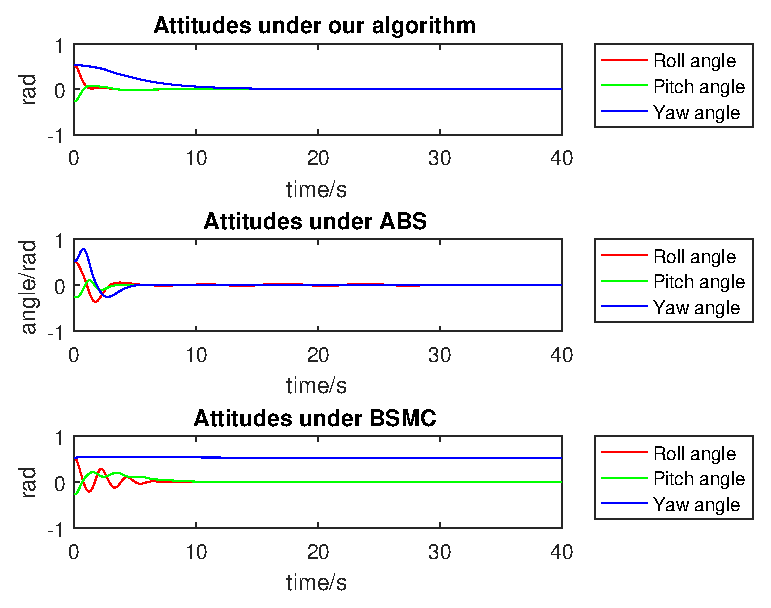
\includegraphics[width=0.45\textwidth]{figure/chap03/case0s-attitudes.eps}
    \bicaption[fig:case0s-locusandattitudes]{初始状态1轨迹图与姿态角对比}{初始状态1轨迹图与姿态角对比}{Fig.}{Trajectories and attitudes compare no disturbance: Case 1}
\end{figure}
\begin{figure}[!h]
    \centering
    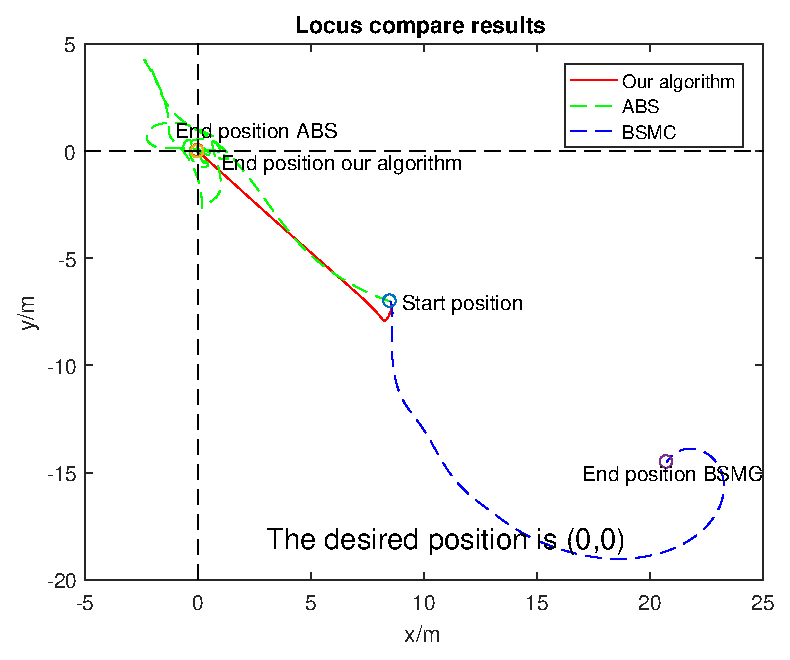
\includegraphics[width=0.45\textwidth]{figure/chap03/case0-locus.eps}
    \hspace{1em}
    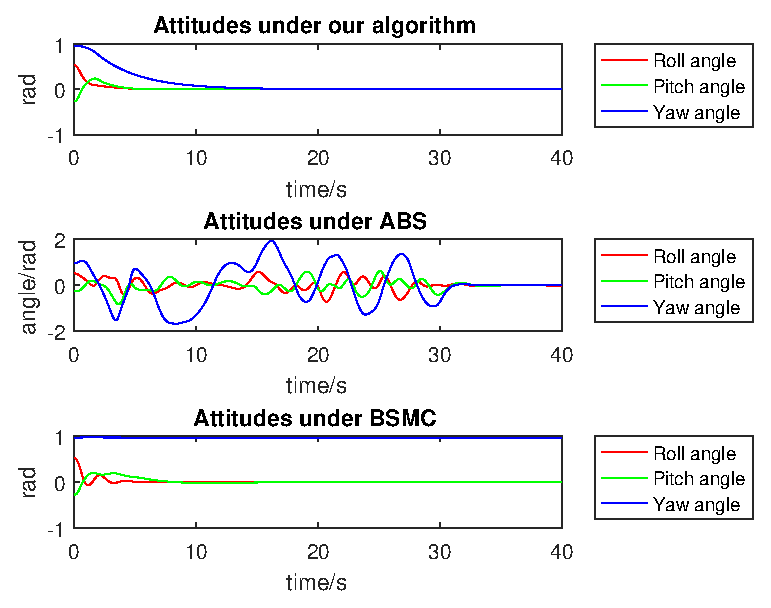
\includegraphics[width=0.45\textwidth]{figure/chap03/case0-attitudes.eps}
    \bicaption[fig:case0-locusandattitudes]{初始状态2轨迹图与姿态角对比}{初始状态2轨迹图与姿态角对比}{Fig.}{Trajectories and attitudes compare no disturbance: Case 2}
\end{figure}

图\newref{fig:case0s-locusandattitudes}与\newref{fig:case0-locusandattitudes}给出了两种初始状态下三种算法的浮空器路径、姿态角对比。从结果我们可以看出来本章\newref{sec:3algo}节的算法与文献\citen{han2015adaptive}中的算法都能很好地完成飞艇姿态稳定。文献\citen{Yang2016Positioning}的算法并不能在六自由度的情形下控制水平位置和偏航角。


\begin{comment}
\begin{figure}[!h]
    \centering
    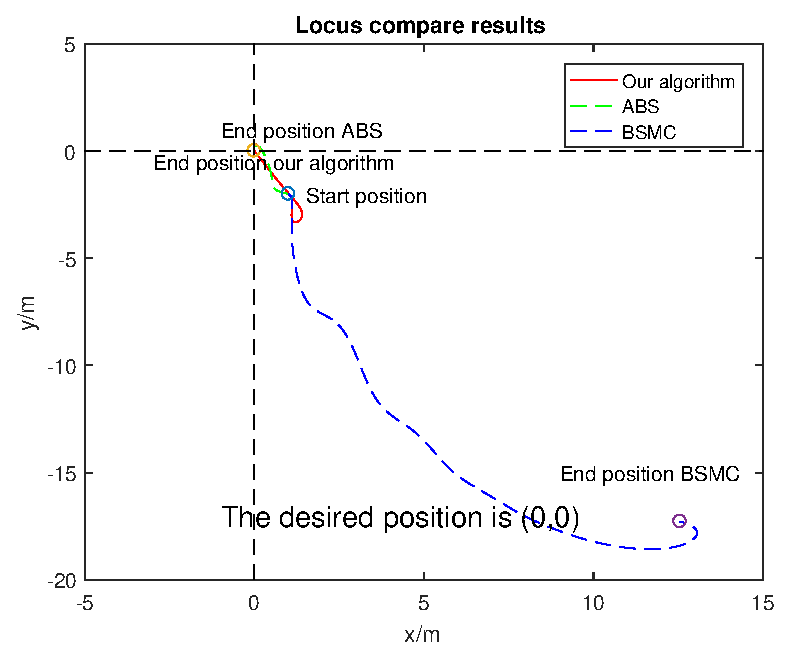
\includegraphics[width=0.7\textwidth,clip]{figure/chap03/case0s-locus.eps}
    \bicaption[fig:case0s-locus]{初始状态1轨迹图对比}{初始状态1轨迹图对比}{Fig.}{Trajectories compare with smaller initial bias and no disturbance: Case 1}
\end{figure}
\begin{figure}[!h]
    \centering
    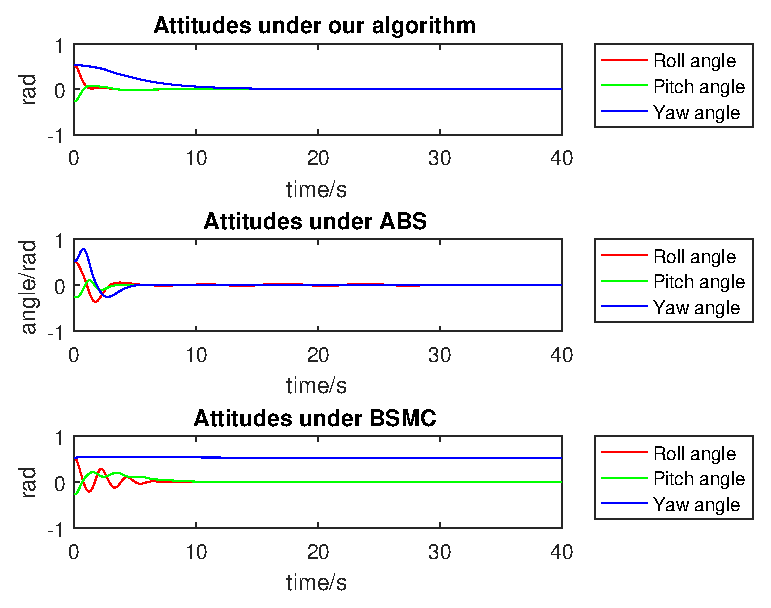
\includegraphics[width=0.8\textwidth,clip]{figure/chap03/case0s-attitudes.eps}
    \bicaption[fig:case0s-attitudes]{初始状态1姿态角对比}{初始状态1姿态角对比}{Fig.}{Attitudes with smaller initial bias and no disturbance}
\end{figure}
\begin{figure}[!h]
    \centering
    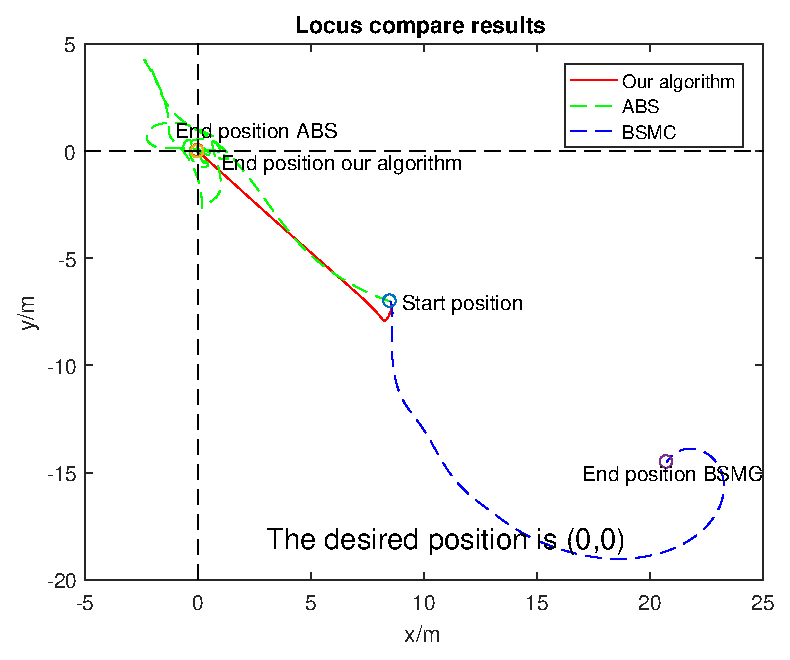
\includegraphics[width=0.45\textwidth,clip]{figure/chap03/case0-locus.eps}
    \bicaption[fig:case0-locus]{初始状态2轨迹图对比}{初始状态2轨迹图对比}{Fig.}{Trajectories compare with smaller initial bias and no disturbance: Case 2}
\end{figure}
\begin{figure}[!h]
    \centering
    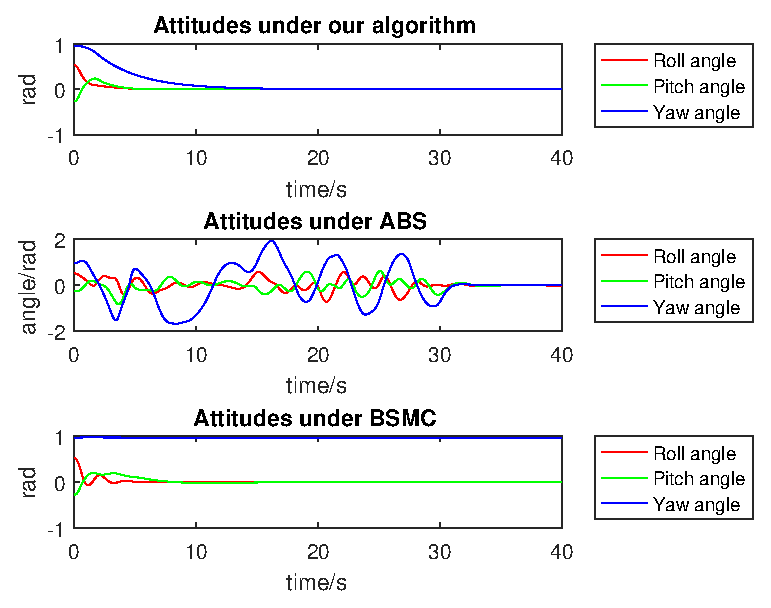
\includegraphics[width=0.45\textwidth,clip]{figure/chap03/case0-attitudes.eps}
    \bicaption[fig:case0-attitudes]{初始状态2姿态角对比}{初始状态2姿态角对比}{Fig.}{Attitudes with smaller initial bias and no disturbance: Case 2}
\end{figure}
\end{comment}

\subsection{仿真2:有扰动情况,自适应滑模抗扰动算法}\label{sec:sim3-2}
本次仿真中,浮空器的初始状态与表\newref{tab:initstate0}的相同,添加的扰动在表\newref{tab:distur1}中给出,其中$X$是服从正态分布的随机变量,满足$X\sim\mathcal{N}(0,1)$。
\begin{table}[htp]
    \centering
    \bicaption[tab:distur1]{仿真2中的扰动}{仿真2中的扰动}{Table}{The disturbances in simulation 2}
    \vspace{0.5em}
    \begin{tabular}{cl}
        \toprule
        扰动变量&扰动值  \\
        \midrule
        $m_{11}$/kg&$10.8147+10\mathrm{sin}(t)$\\
        $m_{22}$/kg&$10.8147+10\mathrm{cos}(t)$\\
        $m_{55}$/kg&$19.3024-50\mathrm{cos}(t)$\\
        $C_x$&$C_x+0.5X$\\
        \bottomrule
    \end{tabular}    
\end{table}

浮空器轨迹的仿真结果在图\newref{fig:case1-locus}中给出。姿态角、速度、角速度的对比分别在图 \ref{fig:case1-attitudes}到\ref{fig:case1-angularvelocities}中给出。 图 \ref{fig:case1-inputAS}到\ref{fig:case1-inputBSMC} 给出了不同算法的控制输入。

\begin{figure}[!htp]
    \centering
    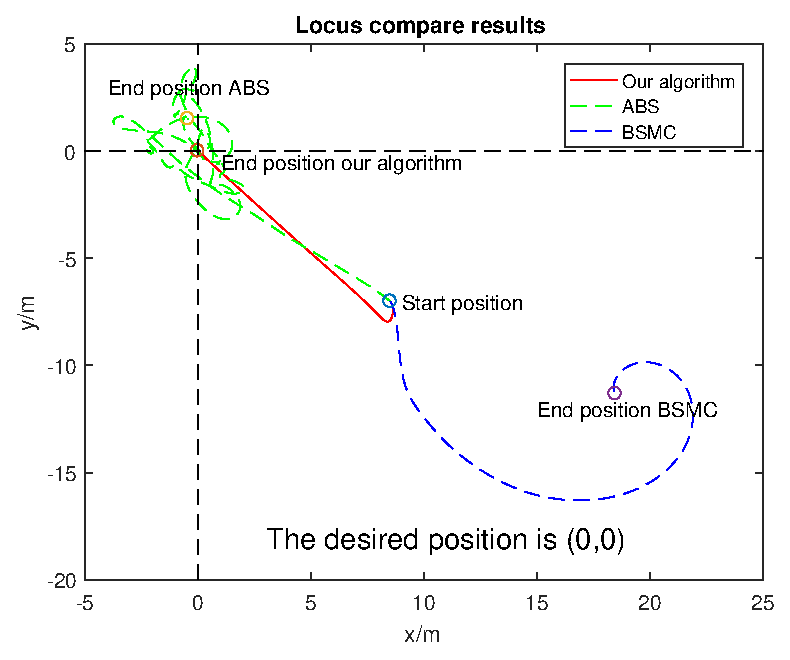
\includegraphics[width=0.7\textwidth]{figure/chap03/case1-locus.eps}
    \bicaption[fig:case1-locus]{仿真2轨迹对比}{仿真2轨迹对比}{Fig.}{Trajectories compare with disturbance under simulation 2}
\end{figure}
\begin{figure}[!htp]
    \centering
    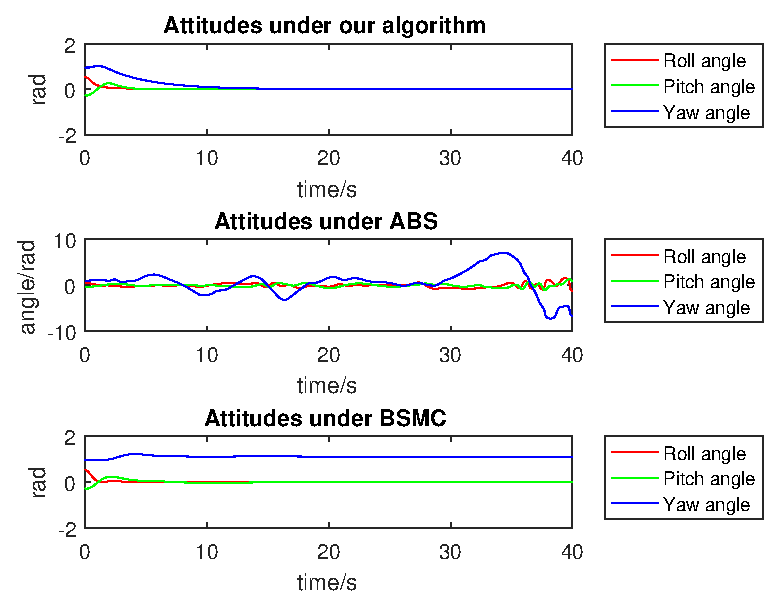
\includegraphics[width=0.7\textwidth,clip]{figure/chap03/case1-attitudes.eps}
    \bicaption[fig:case1-attitudes]{仿真2姿态角对比}{仿真2姿态角对比}{Fig.}{Attitudes compare with disturbance under simulation 2}
\end{figure}
\begin{figure}[!htp]
    \centering
    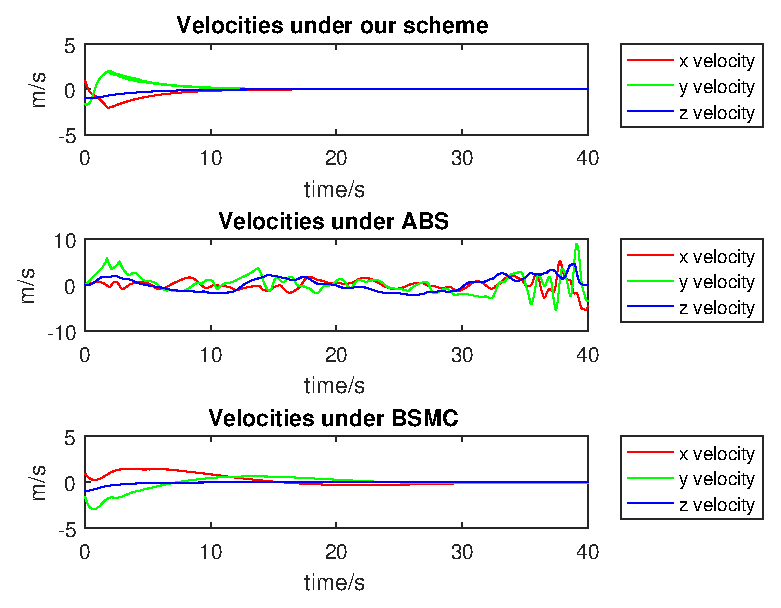
\includegraphics[width=0.7\textwidth,clip]{figure/chap03/case1-velocities.eps}
    \bicaption[fig:case1-velocities]{仿真2浮空器速度对比}{仿真2浮空器速度对比}{Fig.}{Attitudes compare with disturbance under simulation 2}
\end{figure}
\begin{figure}[!htp]
    \centering
    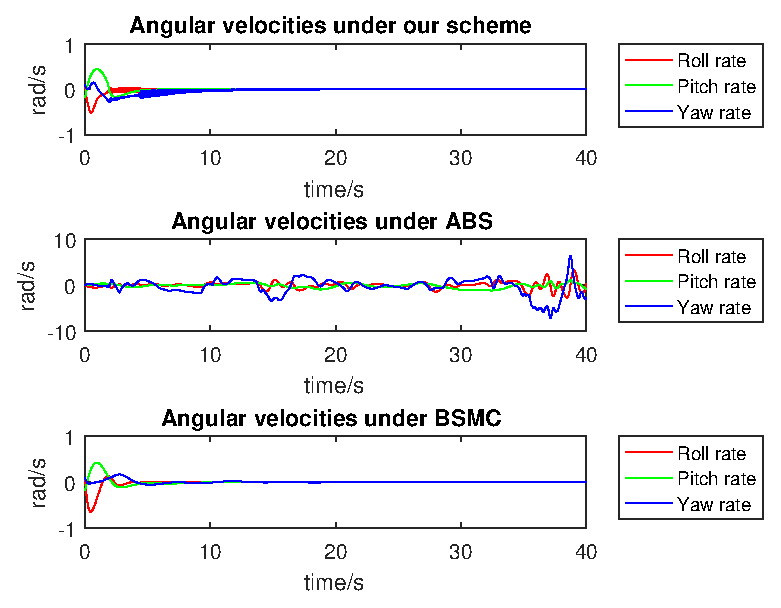
\includegraphics[width=0.7\textwidth,clip]{figure/chap03/case1-angularvelocities.eps}
    \bicaption[fig:case1-angularvelocities]{仿真2浮空器角速度对比}{仿真2浮空器角速度对比}{Fig.}{Angular velocities compare with disturbance under simulation 2}
\end{figure}
\begin{figure}[!htp]
    \centering
    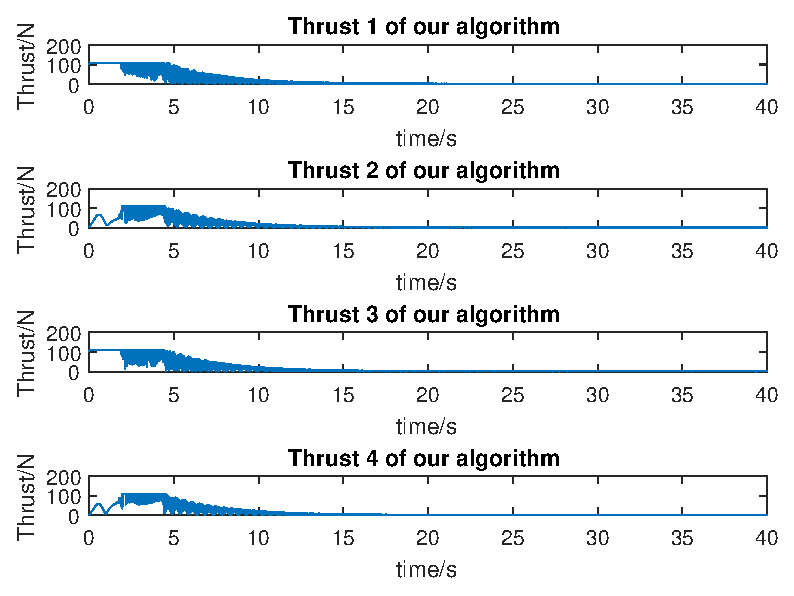
\includegraphics[width=0.7\textwidth,clip]{figure/chap03/case1-inputAS.eps}
    \bicaption[fig:case1-inputAS]{仿真2本文\newref{sec:3algo}算法执行机构输出}{仿真2本文\newref{sec:3algo}算法执行机构输出}{Fig.}{Thrust input forces of algorithm in \newref{sec:3algo} under simulation 2}
\end{figure}
\begin{figure}[!htp]
    \centering
    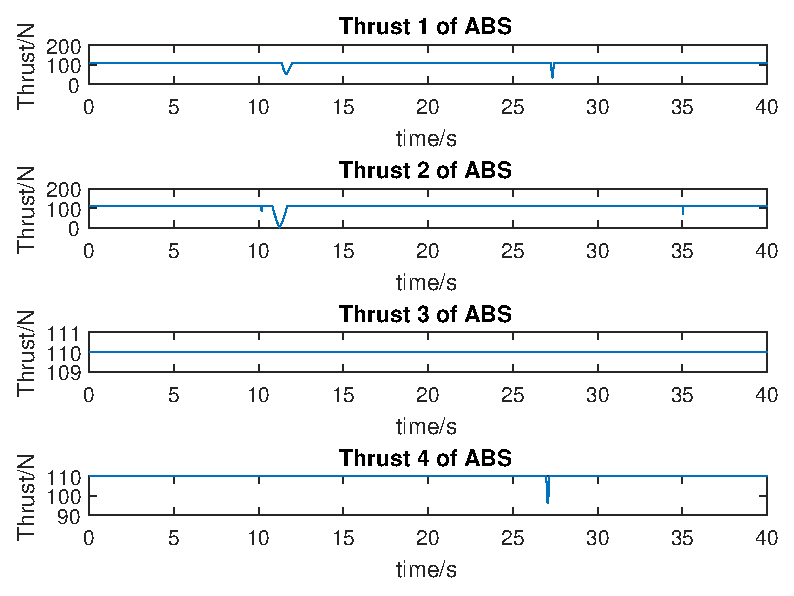
\includegraphics[width=0.7\textwidth,clip]{figure/chap03/case1-inputABS.eps}
    \bicaption[fig:case1-inputABS]{仿真2 ABS算法执行机构输出}{仿真2 ABS算法执行机构输出}{Fig.}{Thrust input forces of ABS algorithm\cite{han2015adaptive} under simulation 2}
\end{figure}
\begin{figure}[!htp]
    \centering
    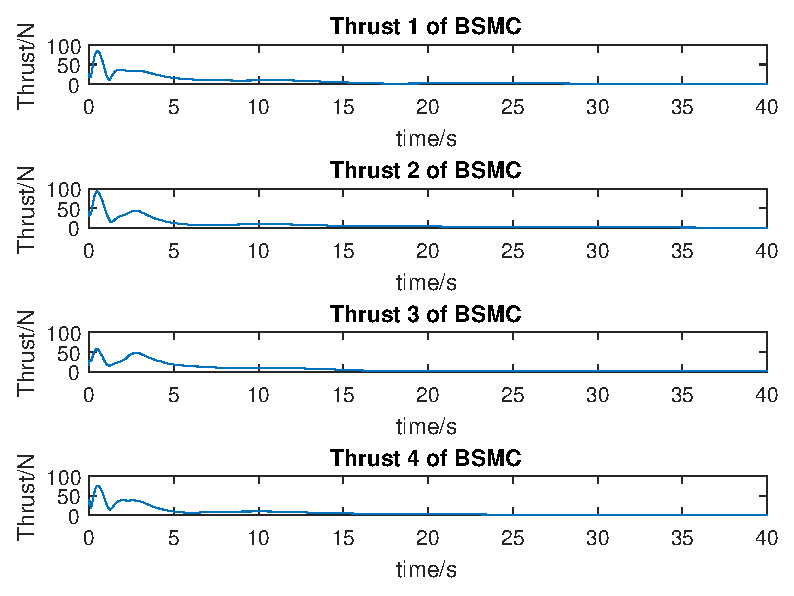
\includegraphics[width=0.6\textwidth,clip]{figure/chap03/case1-inputBSMC.eps}
    \bicaption[fig:case1-inputBSMC]{仿真2 BSMC算法执行机构输出}{仿真2 BSMC算法执行机构输出}{Fig.}{Thrust input forces of BSMC algorithm\cite{Yang2016Positioning} under simulation 2}
\end{figure}

\subsection{仿真3:有扰动,自适应滑模抗扰动考虑饱和算法}\label{sec:sim3-3}

本次仿真中,浮空器的初始状态在表\newref{tab:initstate2}中给出,添加的扰动与表\newref{tab:distur1}中相同。

\begin{table}[htp]
    \centering
    \bicaption[tab:initstate2]{仿真3初始状态}{仿真3初始状态}{Table}{The initial state of the airship under simulation 3}
    \vspace{0.5em}
    \begin{tabular}{cl}
        \toprule
        状态变量&值  \\
        \midrule
        $\mathbf{P}(m)$&$[-8.5,9,4]^T$  \\
        $\mathbf{\Omega}$(rad)&$[\pi/6,-\pi/12,\pi/3]^T$  \\
        $\mathbf{v}$(m/s)&$[1,-1.5,-1]^T$  \\
        $\mathbf{w}$(rad/s)&$[0.1,-0.2,0.1]^T$\\
        \bottomrule
    \end{tabular}    
\end{table}

\begin{figure}[!htp]
    \centering
    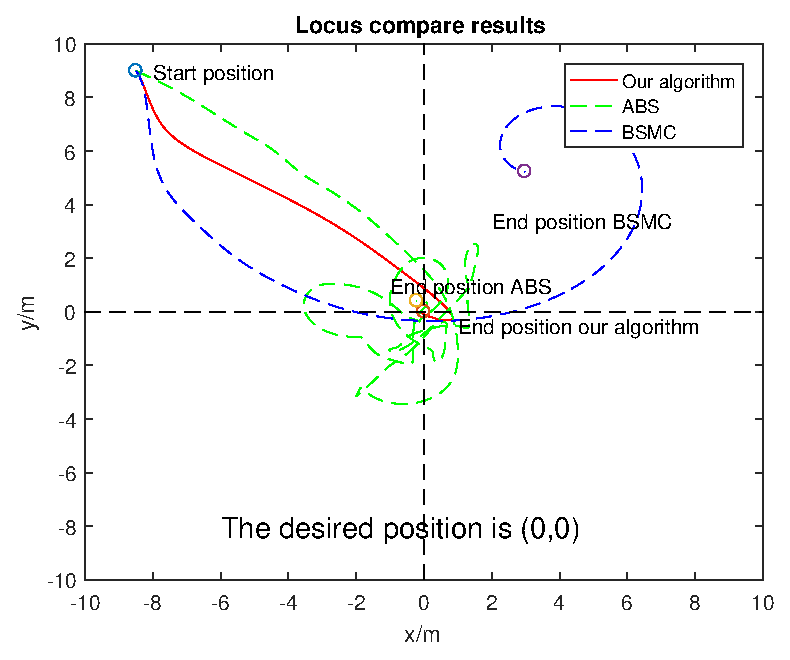
\includegraphics[width=0.7\textwidth]{figure/chap03/case2-locus.eps}
    \bicaption[fig:case2-locus]{仿真3轨迹对比}{仿真3轨迹对比}{Fig.}{Trajectories compare with disturbance under simulation 3}
\end{figure}
\begin{figure}[!htp]
    \centering
    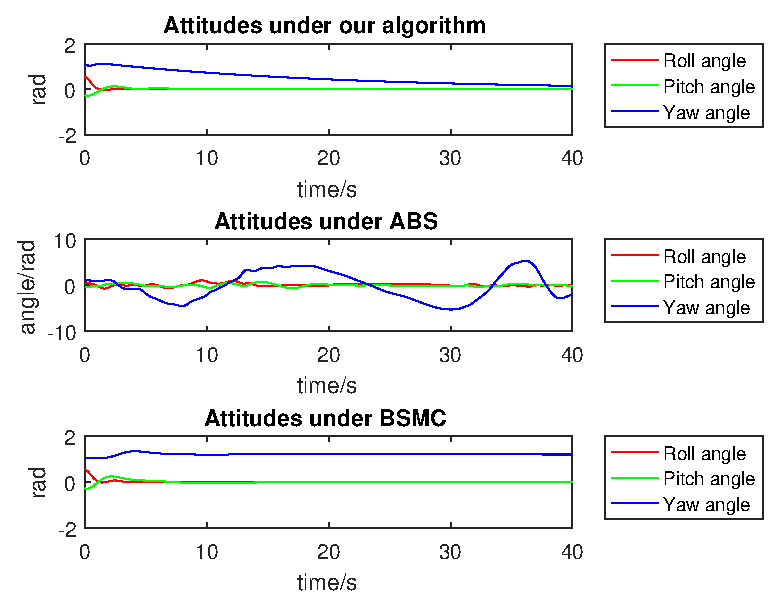
\includegraphics[width=0.7\textwidth,clip]{figure/chap03/case2-attitudes.eps}
    \bicaption[fig:case2-attitudes]{仿真3姿态角对比}{仿真3姿态角对比}{Fig.}{Attitudes compare with disturbance under simulation 3}
\end{figure}
\begin{figure}[!htp]
    \centering
    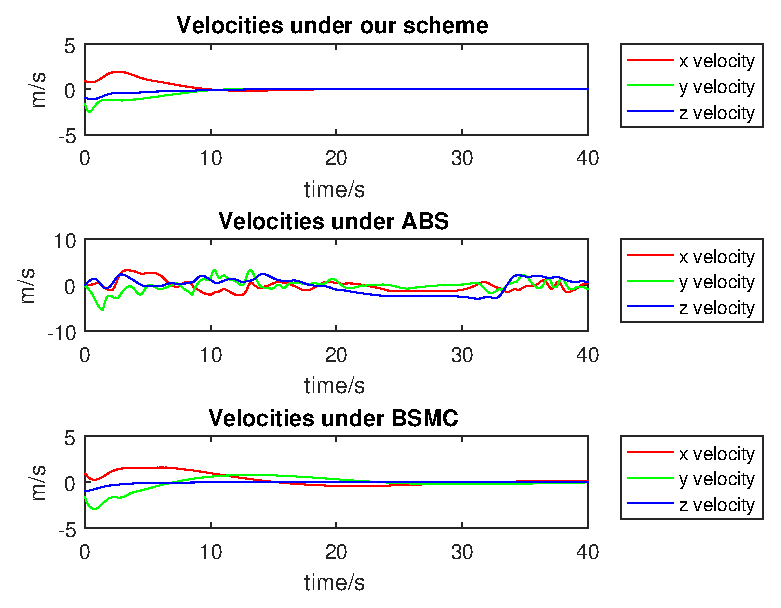
\includegraphics[width=0.7\textwidth,clip]{figure/chap03/case2-velocities.eps}
    \bicaption[fig:case2-velocities]{仿真3浮空器速度对比}{仿真3浮空器速度对比}{Fig.}{Attitudes compare with disturbance under simulation 3}
\end{figure}
\begin{figure}[!htp]
    \centering
    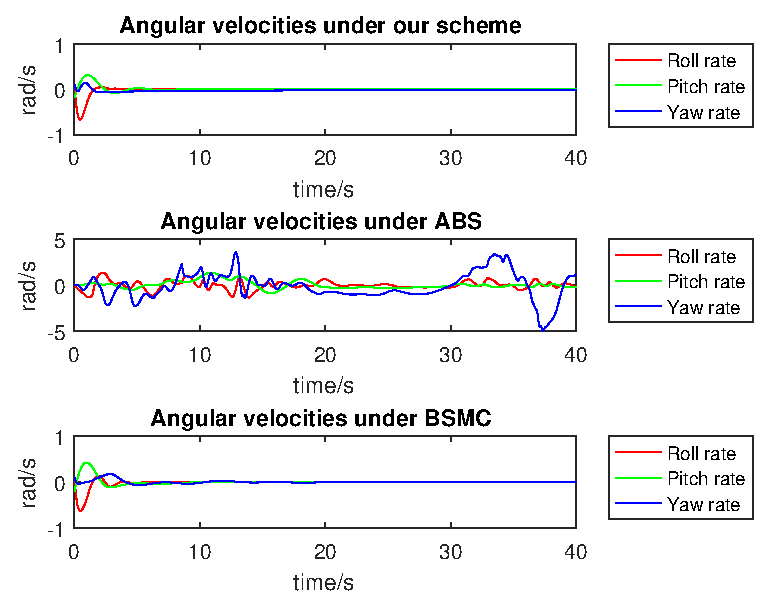
\includegraphics[width=0.7\textwidth,clip]{figure/chap03/case2-angularvelocities.eps}
    \bicaption[fig:case2-angularvelocities]{仿真3浮空器角速度对比}{仿真3浮空器角速度对比}{Fig.}{Angular velocities compare with disturbance under simulation 3}
\end{figure}
\begin{figure}[!htp]
    \centering
    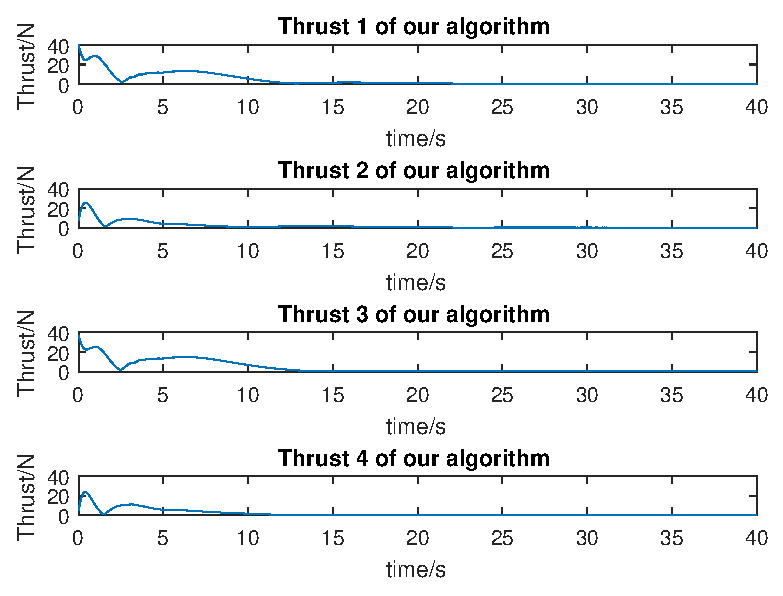
\includegraphics[width=0.7\textwidth,clip]{figure/chap03/case2-inputAS.eps}
    \bicaption[fig:case2-inputAS]{仿真3本文\newref{sec:3algo}算法执行机构输出}{仿真3本文\newref{sec:3algo}算法执行机构输出}{Fig.}{Thrust input forces of algorithm in \newref{sec:3algo} under simulation 3}
\end{figure}
\begin{figure}[!htp]
    \centering
    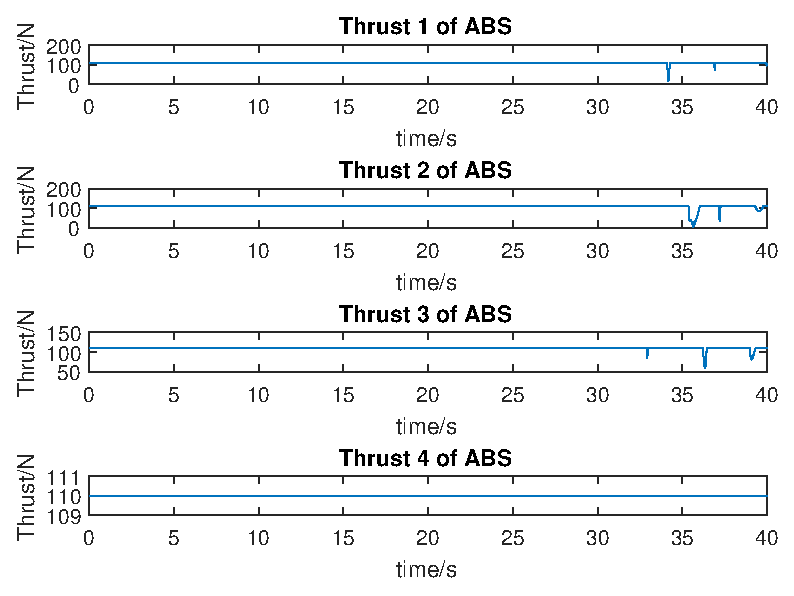
\includegraphics[width=0.7\textwidth,clip]{figure/chap03/case2-inputABS.eps}
    \bicaption[fig:case2-inputABS]{仿真3 ABS算法执行机构输出}{仿真3 ABS算法执行机构输出}{Fig.}{Thrust input forces of ABS algorithm\cite{han2015adaptive} under simulation 3}
\end{figure}
\begin{figure}[!htp]
    \centering
    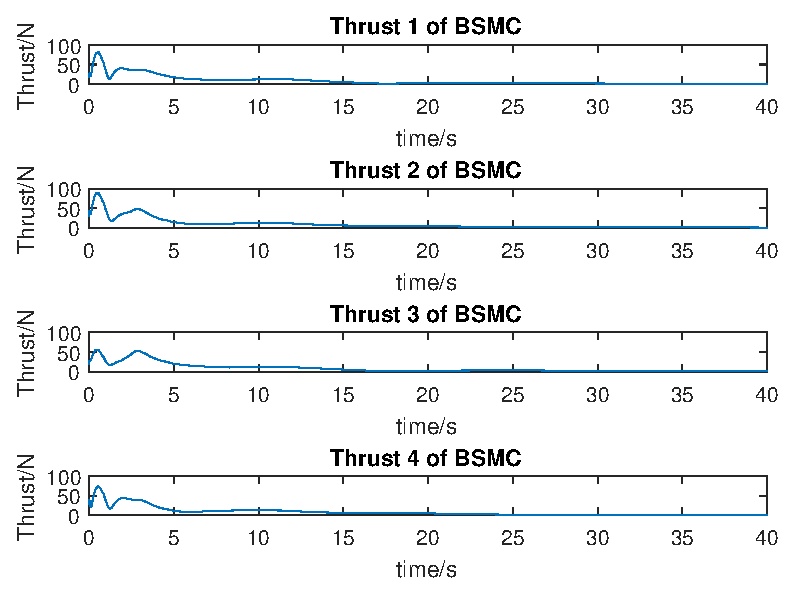
\includegraphics[width=0.6\textwidth,clip]{figure/chap03/case2-inputBSMC.eps}
    \bicaption[fig:case2-inputBSMC]{仿真3 BSMC算法执行机构输出}{仿真3 BSMC算法执行机构输出}{Fig.}{Thrust input forces of BSMC algorithm\cite{Yang2016Positioning} under simulation 3}
\end{figure}

从仿真2和仿真3中,我们可以观察到:
\begin{enumerate}
    \item D.Han的自适应反演算法与浮空器的初始状态高度相关,如果初始状态偏移过大,其算法会剧烈振荡。注意到在D.Han的算法中其执行机构一直在满负荷状态附近工作,这说明其算法虽然具有鲁棒性,但是并不稳定。
    \item 从图\newref{fig:case0s-locusandattitudes}、\newref{fig:case0-locusandattitudes}、\newref{fig:case1-attitudes}和\newref{fig:case2-attitudes}可以看出,Y.Yang的针对三自由度模型的反演滑模算法在处理六自由度模型的时候并不适用。
    \item 本文\newref{sec:3algo}节提出的算法可以很好地处理不不确定性带来的影响,曲线较为平滑,但从图\newref{fig:case1-inputAS}可以看出,其缺陷是执行机构抖震过于明显,且前期输出一直在满负荷附近。但是在\newref{sec:3sat}节的抗饱和算法的结果中(图\newref{fig:case2-inputAS}),执行机构的输出幅度得到了明显的下降,这说明\newref{sec:3sat}提出的抗饱和算法是有效的。
\end{enumerate}

\subsection{仿真4:大偏移长时间仿真}\label{sec:sim3-4}
由于本文提出的自适应滑模算法在系统稳定前会导致估测参数的持续增加,而仿真1至仿真3中采用的都是较小初始偏移量,所以在此增加一例大偏移仿真,以观察系统的收敛时间以及自适应参数增加情况。本次仿真系统的初始状态如表\newref{tab:initstate3}所示,添加扰动与表\newref{tab:distur1}中相同,本次仿真仅采用\newref{sec:3sat}节中的算法,未作对比。

\begin{table}[htp]
    \centering
    \bicaption[tab:initstate3]{仿真4初始状态}{仿真4初始状态}{Table}{The initial state of the airship under simulation 4}
    \vspace{0.5em}
    \begin{tabular}{cl}
        \toprule
        状态变量&值  \\
        \midrule
        $\mathbf{P}(m)$&$[500,500,100]^T$  \\
        $\mathbf{\Omega}$(rad)&$[\pi/4,-\pi/3,\pi/3]^T$  \\
        $\mathbf{v}$(m/s)&$[8,-10,-8]^T$  \\
        $\mathbf{w}$(rad/s)&$[0.3,-0.4,0.3]^T$\\
        \bottomrule
    \end{tabular}    
\end{table}

\begin{figure}[!htp]
    \centering
    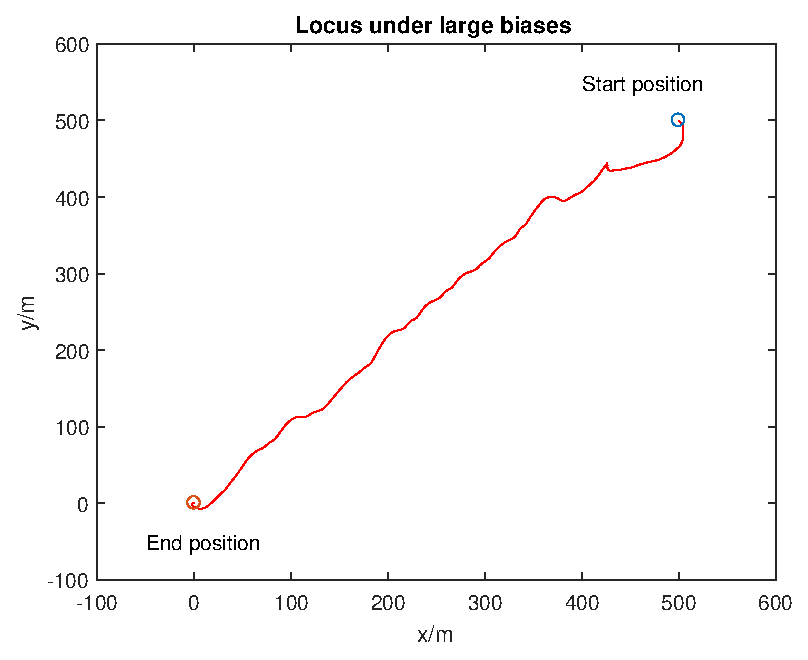
\includegraphics[width=0.7\textwidth]{figure/chap03/case3-locus.eps}
    \bicaption[fig:case3-locus]{仿真4轨迹对比}{仿真4轨迹对比}{Fig.}{Trajectories under simulation 4}
\end{figure}
\begin{figure}[!htp]
    \centering
    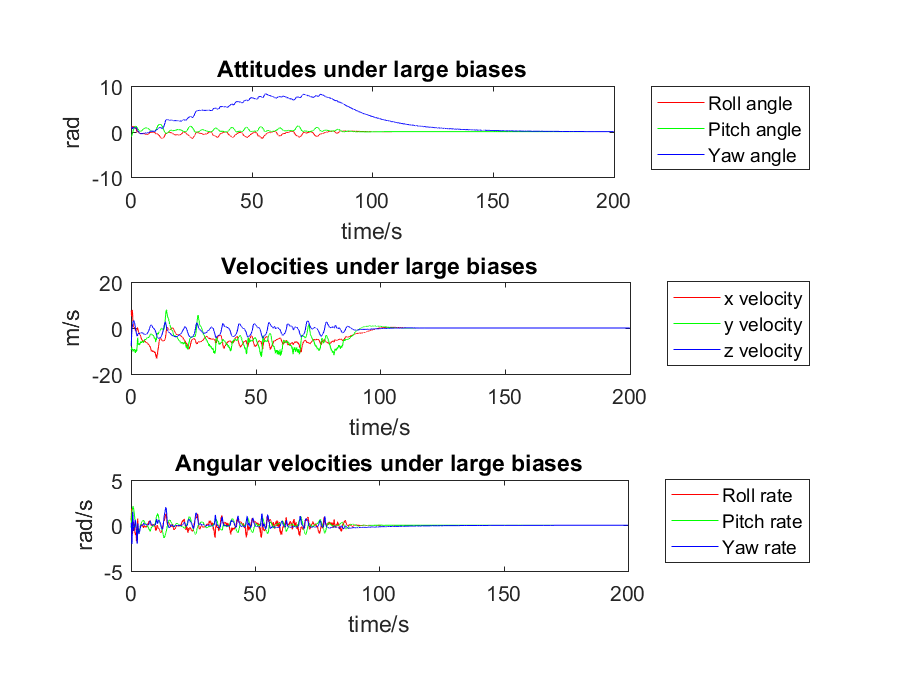
\includegraphics[width=0.7\textwidth,clip]{figure/chap03/case3-states.eps}
    \bicaption[fig:case3-states]{仿真4浮空器各状态}{仿真4浮空器各状态}{Fig.}{Airship states under simulation 4}
\end{figure}
\begin{figure}[!htp]
    \centering
    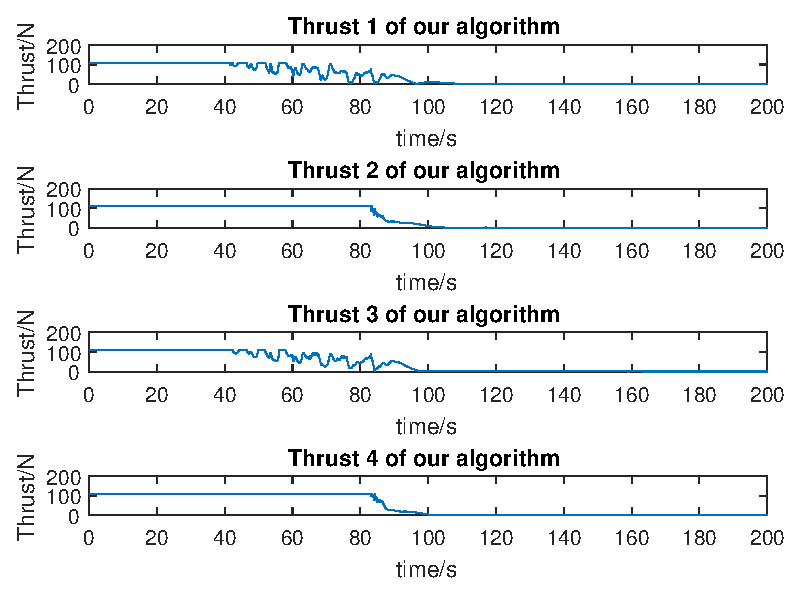
\includegraphics[width=0.7\textwidth,clip]{figure/chap03/case3-inputAS.eps}
    \bicaption[fig:case3-inputAS]{仿真4浮空器执行机构输出大小}{仿真4浮空器执行机构输出大小}{Fig.}{Thrust input forces under simulation 4}
\end{figure}
\begin{figure}[!htp]
    \centering
    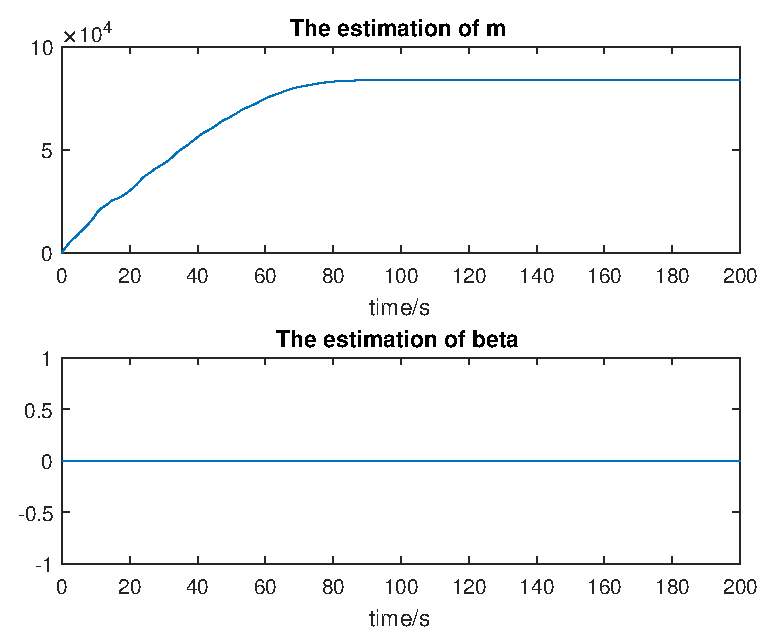
\includegraphics[width=0.7\textwidth,clip]{figure/chap03/case3-paraest.eps}
    \bicaption[fig:case3-paraest]{仿真4自适应参数估计}{仿真4自适应参数估计}{Fig.}{Adaptive parameters estimations under simulation 4}
\end{figure}

从图\newref{fig:case3-locus}至\newref{fig:case3-states}可以看出浮空器大约在90秒的时候回到预定地点保持稳定。图\newref{fig:case3-paraest}说明参数$\hat{\beta}$是稳定的,$\hat{m}$在系统尚未到达滑模面之前是急剧增加的,但在系统接近稳定点的时候就趋于平滑。调节参数$p_3$与$p_4$的值可以减缓这个步骤,但是并不能消除参数无限制增加的影响,这也是本算法的一个缺陷,需要在后续研究中加以克服。


\section{本章小结}
本章介绍了一种基于自适应滑模方法的抗参数扰动的容错控制策略,并在提出算法的基础上添加了抗饱和机制。浮空器特有的高附加质量和气动参数不准确问题,给它的稳定控制增加了很大的困难。本章\newref{sec:3algo}节的算法能够在浮空器同时遭到惯性矩阵扰动和气动参数扰动的前提下使其保持稳定;而\newref{sec:3sat}节提出的算法则对\newref{sec:3algo}节的算法进行了改进,添加了抗饱和机制。为了说明算法的有效性,本章在四种情形下分别对算法做了数值仿真,并且与已有的浮空器鲁棒控制算法进行了对比。